Having constructed an index on a document collection, queries need to 
be matched to documents and a list of answers returned. We need a ranking algorithm based on good mathematical retrieval models to 
retrieve relevant documents at top of the ranking, consequently we will have high effectiveness. 
Three well-known retrieval models~\citep{croft2010search} are: (1) vector space models such as TF-IDF, (2) probabilistic models such as BM25, and Language Models. 

\paragraph{Vector Space Model: TF-IDF}
\ \\
In vector space model, documents and queries are represented by a vector of term weights, and the collection is represented by a matrix of term weights: 
\capstartfalse
\begin{figure}[htpb]
   \centering
   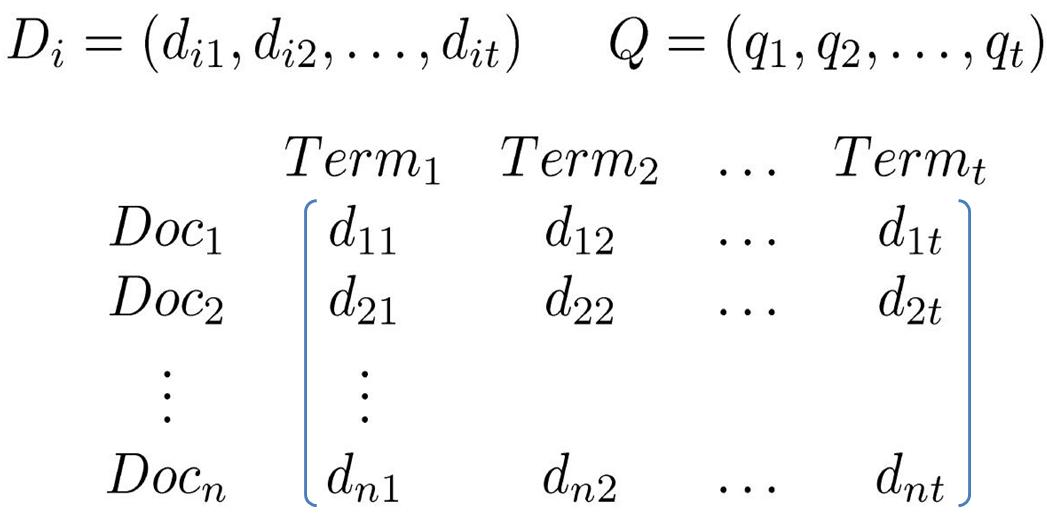
\includegraphics[width=.45\textwidth,height=35mm]{figs/vsm-matrix.jpg}
\end{figure}
\capstarttrue
\FloatBarrier 
\noindent
where , $ D_{i} $ is each document in the collection $ C $ ($ D_{i}\in C $), $ d_{ik} $ is the weight of term $ k $ in document $ D_{i} $, and $ q_{k} $ represents a term in the query $ Q $.
The weighting function multiplies the occurrence of each query term in the document
by the $ idf $ measure, after pivoted normalisation~\citep{bache2010improving}:
\begin{equation}
d_{ik}=\sum\limits_{q \in Q\cap D}\frac{c(q_{k},Di).idf_{k}(q)}{(1-b)+b.\frac{|D|}{avdl}}
\label{eq:tfidf}
\end{equation}
where, $ |D| $ is the size of the document and $ avdl $ is the average document length, $ tf_{ik}(q)=c(q_{k},Di)$ is the number of occurrence of k-th query term in a document $ D_{i} $, and , and inverse document frequency measures importance in the collection: 
\begin{equation}
idf_{k}(q)=\log\frac{N+1}{df(q_{k})}
\label{eq:idf}
\end{equation}
where, $ df(q_{k}) $ is the number of documents in the collection which contain at least one occurrence of $ q $, and $ N $ is the number of documents in the collection. 
This model scores a document higher if more query terms are present or these terms are rarer in the collection. The parameter $ b $ is set to 0.75 to be the same as the BM25 model below.
\paragraph{Probabilistic Models: BM25}
\ \\
BM25 is popular and effective ranking algorithm based on binary independence model. Equation (\ref{eq:idf}) can be improved by factoring in the frequency of each term and document length - it is called Okapi weighting:
\begin{equation}
d_{ik}=\sum\limits_{q \in Q\cap D}\log\frac{N+1}{df(q)}.\frac{(k_{1}+1)c(q,D)}{k_{1}((1-b)+b.\frac{|D|}{avdl})+c(q,D)}
\label{eq:idfbm25}
\end{equation}
The variable $ k_{1} $ is a positive tuning parameter that calibrates the document term frequency scaling. A $ k_{1}=0 $  corresponds to a binary model (no term frequency), and a large value corresponds to using raw term
frequency. $ b $ is another tuning parameter ($ 0 \leq b \leq 1 $) which determines the scaling by document length: $ b = 1 $ corresponds to fully scaling the term weight by the document length, while $ b = 0 $ corresponds to no length normalization. \\\\
If the query is long, then we might also use similar weighting for query terms. This is appropriate if the queries are paragraph long information needs, but unnecessary for short queries.
\begin{equation}
d_{ik}=\sum\limits_{q \in Q\cap D}\log\frac{N+1}{df(q)}.\frac{(k_{1}+1)c(q,D)}{k_{1}((1-b)+b.\frac{|D|}{avdl})+c(q,D)}.\frac{(k_{3}+1)c(q,Q)}{k_{3}+c(q,Q)}
\label{eq:idfbm25}
\end{equation}
with $ c(q,Q) $ being the frequency of term $ q $ in the query $ Q $, and $ k_{3} $ being another positive tuning parameter that this time calibrates term frequency scaling of the query. In the equation presented, there is no length normalization of
queries because retrieval is being done with respect to a single fixed query. The tuning parameters of these formulas should ideally be set to optimize performance on a development test collection. That is, we can search for values of these parameters that maximize performance on a separate development test collection (either manually or with optimization methods such as grid search or something more advanced), and then use these parameters on the actual test collection. In the absence of such optimization, experiments have shown reasonable values are to set $ k_{1} $ and $ k_{2} $ to a value between 1.2 and 2, and b = 0.75~\citep{manning2008introduction}.

\paragraph{Language Models with Terms Smoothing}
\ \\
The basic idea behind the \textit{Language Modelling} approach is to estimate a language model for each document, and rank documents by the likelihood of the query according to the estimated language model. Here terms are assumed to occur independently, and the probability is the product of the individual query terms given the document model $ M_{D} $ of document $ D $:
\begin{equation}
\label{eq:multinomial}
 P(Q|M_{D}) = \prod\limits_{q\in Q} P(q|M_{D}) 
\end{equation}

\begin{equation}
\label{eq:multinomial}
 P(q|M_{D}) = \frac{c(q,D)}{|D|}
\end{equation}

The overall similarity score for the query and the document could be zero if some of query terms do not occur in the document. However, it is not sensible to rule out a document just because a single query term is missing. For dealing with this, language models make use of smoothing to balance the probability mass between occurrences of terms in documents, and terms not found in the documents.
\\\\
\textit{Jelinek-Mercer smoothing.} Jelinek-Mercer smoothing language model~\citep{zhai2004study} combines the relative frequency of a query term $ q\in Q $ in the document $ D $ with the relative frequency of the term in the collection (\textit{C}) as a whole. With this approach, the maximum likelihood estimate is moved uniformly toward the collection model probability $ P(q|C) $:
\begin{equation}
P(q|M_{D}) = (1-\lambda)\frac{c(q,D)}{|D|}+\lambda P(q|C) 
\label{eq:jmsmoothing}
\end{equation} 
$ c(q,D) $ represents the frequency of term $ q $ in document $ D $. The optimal value of $ \lambda $ depends on both the collection and the query. It is normally suggested as ($ \lambda = 0.1$) for title queries and ($ \lambda = 0.7$) for long queries.
\\\\
\textit{Dirichlet (Bayesian) smoothing (DirS).} As long documents allow us to estimate the language model more accurately, Dirichlet smoothing ~\citep{zhai2004study} smooths them less. If we use the multinomial distribution to represent a language model, the conjugate prior of this distribution is the Dirichlet distribution. This gives:
\begin{equation}
\label{eq:bayessmoothing}
 P(q|M_{D}) = \frac{c(q,D) + \mu P(q|C)}{|D| + \mu}
\end{equation} 

The formula assign negative score to documents that contain the term, but with fewer occurrence than predicted by the collection language model. As $ \mu $ gets smaller, the contribution from the collection model also becomes smaller, and more emphasis is given to the relative term weighting. Precision is more sensitive to $ \mu $ for long queries, especially when $ \mu $ is small. When $ \mu $ is sufficiently large, long queries perform better than short queries. The optimal value of $ \mu $ varies from collection to collection, though in most cases, it is around 2000. The performance is more sensitive to smoothing for verbose queries. Long queries also require more aggressive smoothing to achieve optimal performance. 